\documentclass[11pt, a4paper, twoside, openany]{report}
\usepackage[T1]{fontenc}%codifica dei font
\usepackage[utf8]{inputenc}%input encoding
\usepackage[english,italian]{babel}
\usepackage{graphicx}%includere le figure
\usepackage[italian]{varioref}%permette citazioni (con \vref) in cui si inserisce anche il numero di pagina
\usepackage[style=numeric]{biblatex}
\usepackage{xcolor}
\definecolor{darkgreen}{rgb}{0.13, 0.55, 0.13}

\newcommand{\name}{DUILIO }
\newcommand{\software}{Amphitrite }

%Inclusione Package LISTINGS e impostazione delle opzioni
\usepackage{listings}
\lstset{basicstyle=\small\ttfamily,
numbers=left,
tabsize=2,
frame=lines,
keywordstyle=\color{red}\bfseries,
commentstyle=\color{darkgreen},
stringstyle=\color{blue}
}
\addto\captionsitalian{\renewcommand{\lstlistingname}{Codice}}
\addto\captionsitalian{\renewcommand{\lstlistlistingname}{Elenco dei codici}}
\lstset{language=C}

%%%ESEMPIO
%\begin{lstlisting}%
%	[firstline=1, lastline=3, caption={codice}, label={lst:prova}]
%	for (i=1; i<2; ++i){
%		Serial.println("helloworld");//commento
%	}
%\end{lstlisting}

%%%%%%%%%%%%



\bibliography{biblio}
\raggedbottom

\begin{document}
	\begin{abstract}
Il presente fascicolo vuole essere un riassunto delle fasi di costruzioni del primo modello di datalogger utilizzato per le imbarcazioni del Mètis Sailing Unipd e dei suoi successivi sviluppi. Vuole essere un riferimento per chiunque abbia intenzione di portare avanti il progetto e lo sviluppo, voglia costruire un nuovo modello o semplicemente voglia imparare ad utilizzare lo strumento utilizzando questo fascicolo come istruzioni per l'uso.
	\end{abstract}
	
	\tableofcontents
	% !TEX encoding = UTF-8 Unicode
% !TEX TS-program = pdflatex

\chapter{Introduzione}

Questa guida si rivolge sia a chi desidera mettere in funzione \name, sia a chi vuole intraprendere nuovi sviluppi del sistema, per questi ultimi, prima di intraprendere lo studio della presente guida, è fortemente consigliata la lettura di alcune guide di base sull'uso di Arduino, sui protocolli di comunicazione seriale e in particolare l'I$^2$C, lo SPI e la comunicazione seriale UART (sulla quale si deve prestare molta attenzione alla questione byte-ASCII). Infine può tornare utile la conoscenza del protocollo OneWire.

Di fondamentale importanza è avere una basilare esperienza di programmazione e possibilmente un po' di conoscenza del linguaggio C.

Infine è desiderabile, per tutti i lettori, conoscere il modo in cui determinati sensori funzionano, benchè molte feature siano indicate nei capitoli dedicati è sicuramente fondamentale far riferimento ai datasheet per comprenderne meglio le caratteristiche. In particolare è utile conoscere il funzionamento di accelerometri, giroscopi e magnetometri MEMS, come interagire con essi e come si può ricavare l'assetto dai dati 'raw' ottenuti.

Per gli aspiranti alla sola utilizzazione del sistema si consiglia una lettura dei soli capitoli relativi alla messa in funzione dello strumento e all'interpretazione dei dati. Il capitolo su \software darà le istruzioni sull'interfaccia grafica appositamente studiata per interagire con \name per la lettura dei dati in tempo reale e per l'invio di determinati comandi e settaggi.
Questo software, scritto in Python2.7, è in grado anche di leggere i file *.txt salvati su SD dal datalogger.

Per una trattazione sommaria di alcuni argomenti utili si rimanda alle appendici, mentre per quanto concerne lo studio approfondito del filtro utilizzato per ricavare l'assetto si rimanda alle seguenti fonti:

\begin{itemize}
\item Sebastian O.H. Madgwick. An efficient orientation filter for inertial and inertial/magnetic sensor arrays. Rapp. tecn. Bristol University 2010.
\item Sebastian O.H. Madgwick. http://www.c-io.co.uk/open-source-imu-and-ahrs-algorithms
\item R. Vaidyanathan, Sebastian O.H. Madgwick, A.J.L. Harrison. Estimation of IMU and MARG orientation using a gradient descent algorithm. In:Rehabilitation Robotics (ICORR), 2011 IEEE International Conference on (2011), pp 1-7.
\end{itemize}
	% !TEX encoding = UTF-8 Unicode
% !TEX TS-program = pdflatex

\chapter{Obiettivi}

Si è voluto progettare e costruire un apparato elettronico utile per acquisire molteplici informazioni sulle imbarcazioni durante la navigazione. L'utilizzo di questi dati sarà poi da un lato finalizzato al miglioramento tecnico degli equipaggi, dall'altro servirà per affinare le tecniche di progettazione per valutare se effettivamente le barche rispondo secondo quanto voluto in fase di progettazione. Infine, in funzione di un progetto molto più ampio, le rilevazioni potranno essere utili come feedback per l'affinamento delle tecniche di simulazione CFD.

L'interesse nel produrre un sistema a basso costo e completamente customizzabile ci hanno indirizzato verso il mondo Arduino che, almeno in un primo momento, sarà il cervello del nostro apparato. Si prevede in futuro di ampliare il sistema e di conseguenza potrebbe essere utile l'inserimento di sistemi più potenti come ad esempio Raspberry abbinati a microcontrollori eventualmente standalone. La scarsa conoscenza ed esperienza in elettronica e in programmazione ci hanno fatto optare per l'utilizzo di schede preassemblate con una buona quantità di documentazione disponibile


Le funzionalità richieste sono:
\begin{itemize}
\item rilevamento dell'assetto;
\item rilevamento della posizione;
\item rilevamento del vettore velocità (modulo e verso);
\item rilevamento delle condizioni ambientali (vettore veloicità del vento, temperatura);
\item predisposizione per la misura di carichi e deformazioni;
\item salvataggio dati;
\item invio dati in tempo reale (successiva implementazione);
\item schermo per la visualizzazione id informazioni utili;
\end{itemize}
	% !TEX encoding = UTF-8 Unicode
% !TEX TS-program = pdflatex

\chapter{Invio e ricezione dati}
La sintassi generale per l'invio e la ricezione di dati, siano essi comandi o dati rilevati, è la seguente:
\begin{lstlisting}%
	[firstline=1, lastline=3, caption={sintassi per lo scambio seriale di informazioni}, label={lst:stringaFPV}]
	$TYPE,val_1,val_2,...,val_n*checksum\n
\end{lstlisting}
dove \$ è il carattere di inizio stringa, TYPE è un byte che identifica il tipo di stringa che stiamo inviando, dopo la virgola invece vengono inseriti i bytes che formano la stringa. La comunicazione seriale spedisce e riceve un byte per volta, i byte possono contenere informazioni numeriche o caratteri, dipende dal modo in cui vengono poi interpretati.
Nelle appendici è presente una piccola guida sulla codifica ASCII al cui interno è presente la tabella [\ref{fig:tabellaAscii}] che mostra le conversioni nei vari tipi di codifica utilizzata.

\'E evidente che il formato utilizzato per inviare i dati sia del tutto simile alle stringhe NMEA, in questo caso però inviamo i byte in formato 'numerico', cioè il dato che ci arriva è pronto all'uso o al massimo va ricomposto con delle operazioni di Bit Shift per aumentarne la precisione. Questo ci permette di aumentare moltissimo le prestazioni, infatti si prenda ad esempio il valore $255$, il massimo inviabile con un solo byte, se lo inviassimo sotto forma di caratteri dovremmo inviare tre bytes (uno per ogni carattere che compone il numero), facendolo sotto forma di byte riduciamo il peso dell'invio e aumentiamo la velocità di comunicazione.

Si deve però prestare attenzione al tipo di device che abbiamo di fronte, questo è possibile farlo solo qualora si abbia il controllo su entrambi i lati dello scambio di informazioni. Qualora si abbia a che fare con un GPS, per fare un esempio, dobbiamo uniformarci al suo protocollo che invece invia i caratteri singolarmente e quindi per interpretarli in modo corretto è necessario conoscere la codifica ASCII, un approfondimento è presente nelle appendici della guida.

\section{FPV Telemetry}
Lo scambio di informazioni in telemetria è reso possibile attraverso il modulo FPV che lavora a $533MHz$. Lato \name è collegato ad una porta seriale (di default alla numero 3), lato computer invece si collega alla porta USB in quanto il modulo di terra è dotato di un convertitore USB-UART. La seriale lavora a $57600 baud$.

Proprio per questo modulo abbiamo previsto il sistema di comunicazione indicato nel listato \{\ref{lst:stringaFPV}\}.

Al momento il sistema è predisposto per la ricezione di comandi composti da un byte di type e uno di comando, per modificare la lunghezza è sufficiente andare a cambiare il valore della label LENGTH presente nel file Const.h allegato al codice sorgente, il valore li presente tiene conto solo dei byte di comando e non quelli di tipo.

Per evitare sovraccarichi della seriale in accensione, nel caso di temporanee perdite di segnale o interruzione del software è presente un check nel codice di \name che in caso di silenzio prolungato ($60$ secondi attualmente, ma si può modificare attraverso la label $CONNECTION\_TIMEOUT$ In \software è invece presente una funzione automatica che a intervalli predeterminati (attualmente $60$ cicli della funzione che controlla l'orologio, quindi $60s$) invia un byte $\$0,4*4$.

\begin{table}
	\begin{center}
		\begin{tabular}{|l|l|l|}
			\hline
			type byte & command byte & significato\\
			\hline
			\hline
			0 & 0 & errore:\\
			0 & 1 & errore:\\
			0 & 2 & errore:\\
			0 & 3 & errore:\\
			0 & 4 & check connessione\\
			0 & 5 & inizia a salvare e inviare dati\\
			0 & 6 & ferma il salvataggio e l'invio di dati\\
			\hline
		\end{tabular}
	\end{center}
	\caption{Lista dei comandi attualmente disponibili} 
	\label{tab:comandiFPV}
\end{table}

\section{Stringhe Disponibili}
Le tabelle seguenti indicano quali sono e cosa contengono le stringhe disponibili. \'E possibile inviarle sia come byte ascii (generalmente è il metodo usato per salvare su SD), sia come byte numerici (usato per migliorare le prestazioni per l'invio wifi).
La differenza tra i due è che nel secondo caso, per migliorare ulteriormente la prestazione, non sono indicati i 'reference' cioè le parti di stringa che indicano l'unità di misura o l'ordine dei dati. Non è possibile eliminarli dalle stringhe su file di testo per una questione di comprensibilità.

\begin{table}
	\begin{center}
		\begin{tabular}{|l|l|l|}
			\hline
			type string & acronimo\\
			\hline
			\hline
			\$MVUP & Mètis Vela UniPd\\
			\$MVIC & Mètis Vela Infusion Check\\
			\hline
		\end{tabular}
	\end{center}
	\caption{Stringhe ascii disponibili} 
	\label{tab:AsciiNMEA}
\end{table}

\begin{table}
	\begin{center}
		\begin{tabular}{|l|l|l|}
			\hline
			type byte & stringa di riferimento\\
			\hline
			\hline
			1 & \$MVUP\\
			10 &  \$MVIC\\
			\hline
		\end{tabular}
	\end{center}
	\caption{Relativi type byte in telemetria} 
	\label{tab:ByteNMEA}
\end{table}
	
	\appendix
	% !TEX encoding = UTF-8 Unicode
% !TEX TS-program = pdflatex

\chapter{I caratteri ASCII}

\begin{figure}[ht!]
\centering
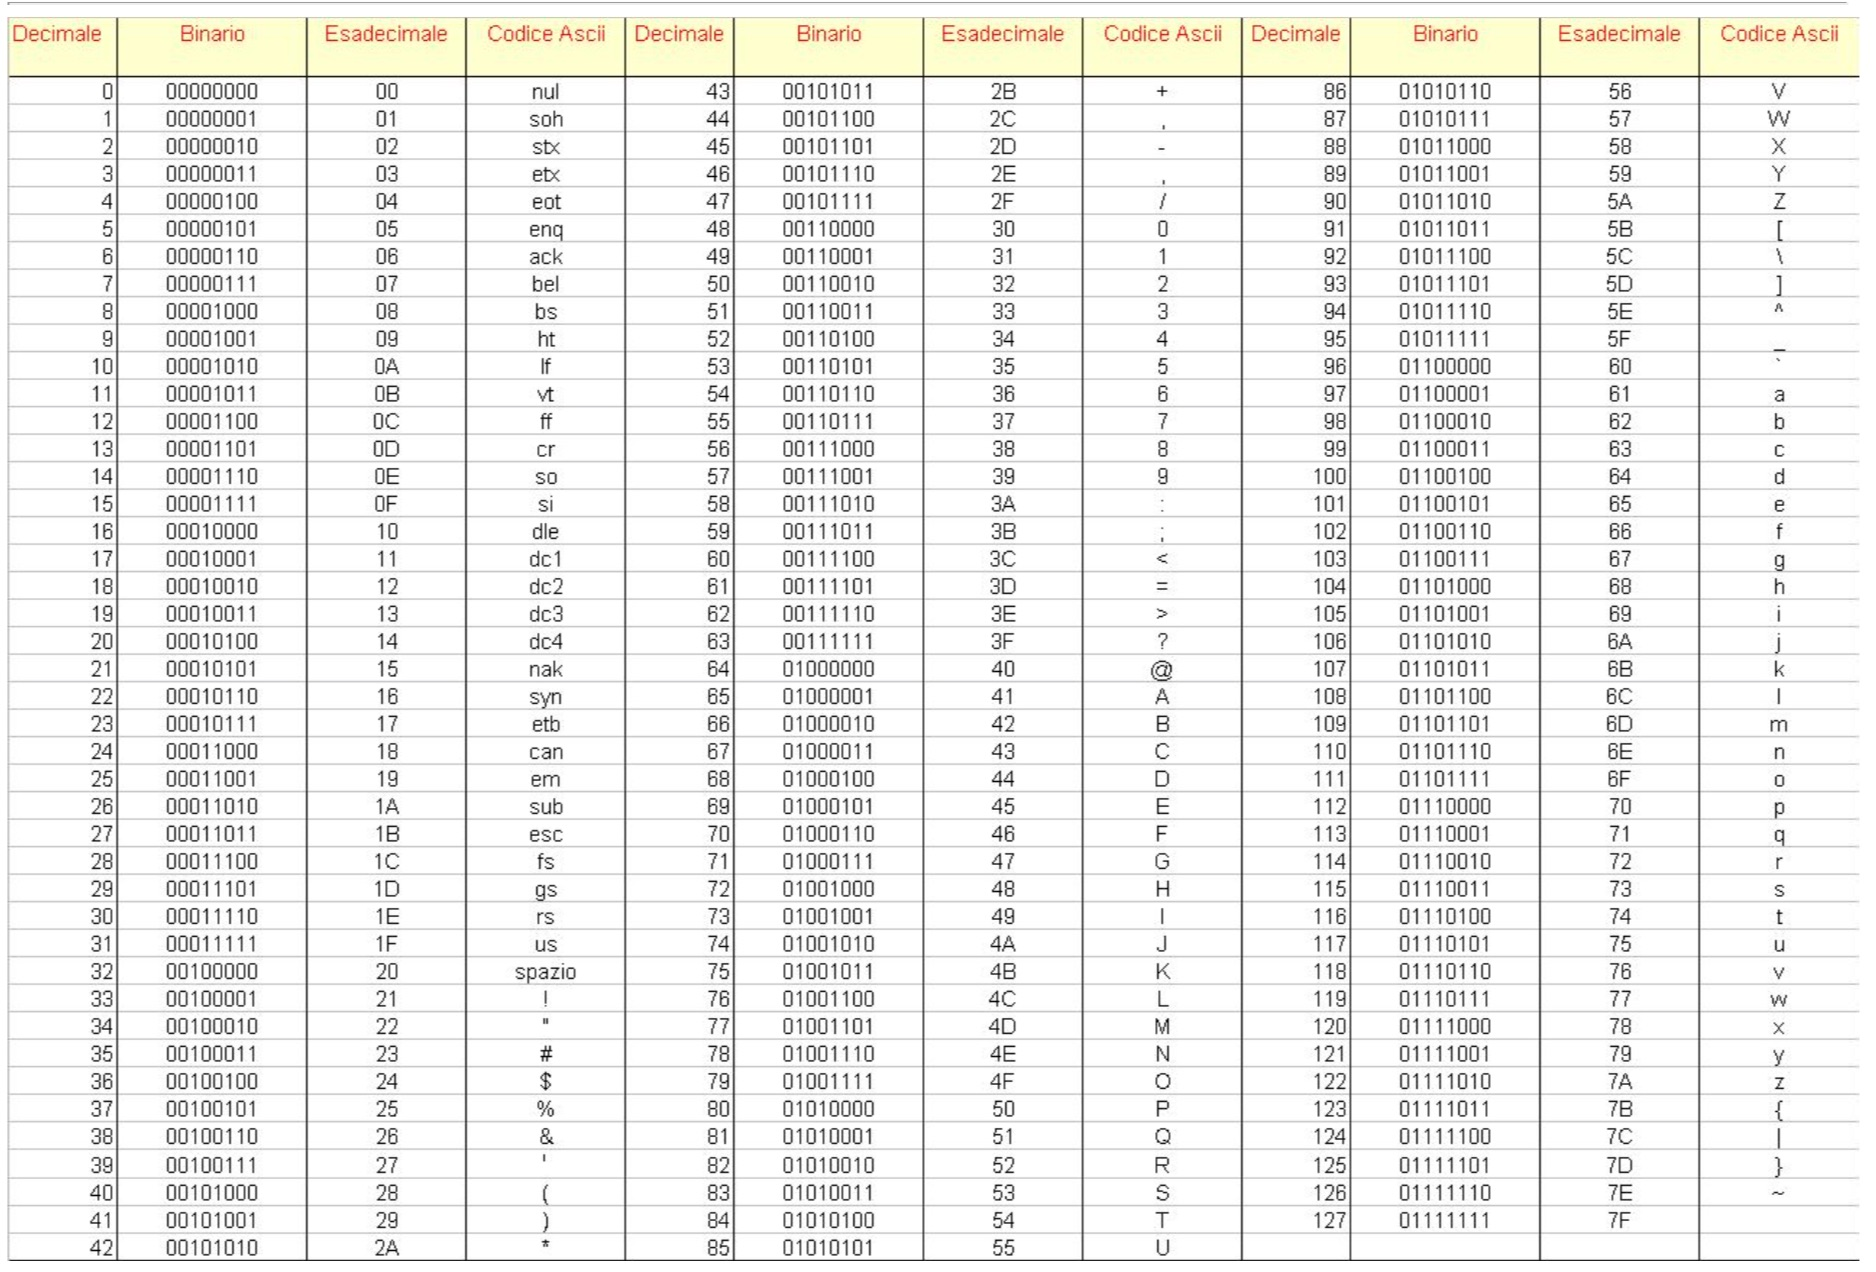
\includegraphics[width=175mm, angle=90]{Appendici/Contenuti/asciiTab.jpg}
\caption{Elenco dei caratteri Ascii e dei corispettivi valori Hex, Bin, Dec \label{fig:tabellaAscii}}
\end{figure}

	

	\nocite{*}
	\printbibliography

	\listoffigures
	\listoftables
	\lstlistoflistings
\end{document}